
%(BEGIN_QUESTION)
% Copyright 2012, Tony R. Kuphaldt, released under the Creative Commons Attribution License (v 1.0)
% This means you may do almost anything with this work of mine, so long as you give me proper credit

Examine the primary and secondary connections on this three-phase transformer bank, and then determine the line voltage to the customer, assuming 12.5 kV line voltage on the distribution power lines.  The schematic diagram shown in the grey box is typical for each of the three transformers:

$$\includegraphics[width=15.5cm]{i01041x01.eps}$$

\underbar{file i01041}
%(END_QUESTION)





%(BEGIN_ANSWER)

The transformer primary windings are connected in a Wye configuration, which means each primary winding receives the 7.2 kV phase voltage.  The secondary windings are connected in a Delta configuration, making the secondary line voltage equal to 240 volts.

$$\includegraphics[width=15.5cm]{i01041x02.eps}$$

%(END_ANSWER)





%(BEGIN_NOTES)



%INDEX% Electronics review: 3-phase electrical power 
%INDEX% Electronics review: AC transformer circuit
%INDEX% Process: AC power distribution system (transformer)

%(END_NOTES)


